\documentclass[]{article}
\usepackage[ngerman]{babel}
\usepackage{graphicx}
\usepackage{amsmath}
\usepackage[utf8]{inputenc}
\usepackage[T1]{fontenc}
\usepackage[ngerman]{babel}
\usepackage{courier}
%opening
\title{Erfahrungen aus der Erstellung des Projektes \glqq ThermoAmpel\grqq{} für das Seminar \glqq Mikrocontrollerschaltungen - Realisierung in Hard- und Software\grqq}
\author{Ilhan Aydin, Lev Perschin}

\begin{document}

\maketitle
\newpage
\begin{abstract}

\end{abstract}
\newpage
\section{Erste Erfahrungen/Schritte}
Wir, Ilhan und Lev, hatten wenig Vorwissen in diesem Bereich. Wir haben noch nie ein Schaltplan erstellt, die Komponenten auf dem Board verteilt, es gedruckt, bestückt und anschließend programmiert. Das Wissen, welches wir hatten, waren Kenntnisse aus der Vorlesung \glqq Technische Informatik\grqq{} und ähnliche.


\section{Schaltplan}
\begin{itemize}
	\item Auswahl der richtigen Teile - größtenteils von PDF übernommen
	\item Berechnung von LED Widerstanden
	\item Übersichtlichkeit wichtig
	\item Offene Pins mit einem Stecker(?) versehen, damit man sie in Zukunft leichter verwenden kann
\end{itemize}
\section{Board}
\begin{itemize}
	\item Positionierung der Teile - im Nachhinein vielleicht wie es am schlausten wäre?
	\item VDD Leitung etwas dicker
	\item Groundpins mit Verbindung zur Groundplate richtig einstellen
	\item Nach dem Löten mit Messgerät schauen, ob Verbindungen da sind wo sie sein sollten und nicht da sind wo sie nicht sein sollten
\end{itemize}
\section{Software}
Dieser Abschnitt beschreibt unsere Herangehensweise an das Programmieren des Mikrocontrollers. Ausgehend davon, dass in der Platine alles korrekt verschaltet ist, kann man mit dem Programmieren beginnen. Wir haben dafür einen Programmer von DIAMEX verwendet. Vorteil bei diesem Programmer ist, dass es die Platine mit 5V versorgen kann, sodass man beim Programmieren die Platine nicht extra an eine Stromversorgung anschließen muss. 
***-HIER ROUTINE ZUM ÜBERPRÜFEN DER ATMELSTUDIO ERKENNUNG -> Probleme mit 5V usw -> Erdungspins nicht korrekt -> wurde ersichtlich, nach dem schreiben des LED programms.***
Zum Testen, ob der Mikrocontroller mit unserem Programm überschrieben worden ist, haben wir vorerst ein einfaches Programm geschrieben, welches die LEDs ansteuert. Nachdem die oben genannten Schwierigkeiten überwunden waren und der Mikrocontroller das LED-Programm richtig ausgeführt hat, begannen wir mit der Implementation unserer Aufgabe. Die Aufgabe bestand daraus mittels eines Temperatur- und Luftfeuchtigkeitsensors die Temperatur und Luftfeuchtigkeit auszulesen und über die UART-Schnittstelle auszugeben. Zusätzlich lassen wir über die LEDs anzeigen, ob die Temperator und Luftfeuchtigkeit im guten Bereich liegen. 
\subsection{Ansteuern des Sensors}
Wie man es nicht machen sollte:
Zunächst haben wir probiert, mit dem Sensor über das Two-wire Serial Interface (TWI) zu kommunizieren. Wie man über TWI kommuniziert ist im Datenblatt des Atmega16 ausführlich mit Codebeispielen beschrieben ***(Seite 175 ff.)***. Nach der Implementierung einer Routine zum Kommunizieren über TWI fiel uns auf, dass der Sensor TWI gar nicht unterstützt. Eine andere Lösung musste her.
Wie man es machen sollte:
Wie man mit dem Sensor richtig kommuniziert, steht im Datenblatt des Sensors geschrieben. Dazu sendet man dem Sensor ein Kommando über den SCK- und DATA-Pin des Sensors, wartet auf die Bearbeitung des Kommandos und liest zum Schluss die Antwort aus. 
Das Senden eines Kommandos wird mit über das Senden der folgenden Bitfolge initiiert, welche im Datenblatt auch "`Transmission Start"' genannt wird: 
\begin{figure}[h]
	\centering
	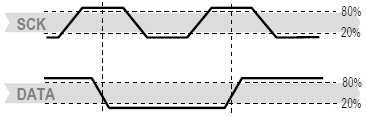
\includegraphics[width=0.5\columnwidth]{transmission_start.png}
	\caption{Transmission Start}
\end{figure}
\\ Um das Senden im Programm zu realisieren setzt man zunächst die Pins, über die SCK und DATA verbunden sind, auf Ausgang. Dann setzt man bei DATA eine 1 und bei SCK eine 0 an, damit der Zustand von DATA mit High und der von SCK mit Low beginnt, wie auch in der Abbildung dargestellt ist. Wie man weiter vorgeht, kann man der Abbildung entnehmen. Wenn der Zustand vom SCK oder DATA von Low auf High wechselt, bedeutet das, dass man an den mit SCK oder DATA verbundenen Port eine 1 anlegt. Der Wechsel von High zu Low entspricht dem anlegen einer 0. Nachdem man Transmission Start übertragen hat, kann man nun ein Kommando übertragen. Um beispielsweise die Temperatur abzufragen, sendet man die Sequenz 00000011. Das Senden geschieht ebenfalls durch das Setzen und Entfernen von Bits am Port von SCK und DATA. Wenn der Sensor ein Kommando erhalten hat, sendet er ein ACK zurück. Zum Überprüfen, ob das Senden des Kommandos erfolgreich war, setzt man DATA auf Eingang und legt eine 1 an, um den internen Pullup-Widerstand zu nutzen. Dies ist nötig, um die vom Sensor gesendeten Bits lesen zu können. Wird DATA vom Sensor aus auf Low gesetzt, hat er das Kommando erhalten. Nun wartet man bis die Messung fertig ist. Der Sensor setzt DATA auf Low, wenn es die Messung beendet hat. Das Lesen der Daten erfolgt Byteweise. Nachdem man ein Byte gelesen hat, sendet man dem Sensor ein ACK und liest danach das nächste Byte aus, falls die Daten eine höhere Genauigkeit als acht Bit haben. Insgesamt liest man drei Bytes aus, wobei letzte Byte die Checksumme beinhaltet. Die Kommunikation endet nach dem Auslesen des dritten Bytes. Man kann sie auch nach dem Lesen des zweiten Bytes beenden, wenn man die Checksumme nicht benötigt. Dazu lässt man DATA nach dem Senden des ACKs auf High. 
\\Beim Kommunizieren ist es wichtig, nicht zu vergessen, dass wenn man etwas senden will, der Port von DATA auf Ausgang und beim Lesen auf Eingang gesetzt werden muss. Zudem sollte man die Häufigkeit der Anfragen auf eine pro Sekunde beschränken, um die vom Sensor abgegebene Wärme zu reduzieren.

\subsection{Auswerten der Daten}
Die Daten, die man vom Sensor erhält, müssen für die Ausgabe umgewandelt werden. Dazu gibt es im Datenblatt des Sensors Formeln, wie zum Beispiel Folgendes für die Berechnung der relativen Luftfeuchtigkeit:
\begin{equation*}
RH_{linear} = c_1 + c_2*SO_{RH} + c_3*SO_{RH}^{2} \left(\%RH\right)\textbf{,}
\end{equation*}
wobei $SO_{RH}$ die vom Sensor ausgelesenen Bits bezeichnet. Wenn $SO_{RH}$ eine Genauigkeit von 12 Bit hat, verwendet man für die Konstanten $c_1$, $c_2$ und $c_3$ folgende Werte: $c_1 = -2.0468$, $c_2 = 0.0367$, $c_3 = -1.5955*10^{-6}$.
Beispielsweise würde die vom Sensor erhaltene Bitfolge "0000 0100 0011 0001" (1073) einer relativen Luftfeuchtigkeit von 35.50\% entsprechen.\\
Die Formel kann man allerdings nicht im Mikrocontroller ohne Weiteres verwenden, da diese Genauigkeiten zum Berechnen erfordert, die der Mikrocontroller nicht aufbringt. Eine Möglichkeit zum Umwandeln der Bits in relative Luftfeuchtigkeit oder Temperatur besteht daraus, die entsprechenden Werte für die relative Luftfeuchtigkeit und der Temperatur für alle Bits vorher auszurechnen und in Form einer Lookup-Tabelle im Programm zu realisieren, damit der Mikrocontroller keine aufwändigen Rechnungen machen muss. Man bräuchte also bei einer Messung mit einer Genauigkeit von 14 Bit eine Lookup-Tabelle mit $2^{14}-1 = 16383$ Einträgen. Um die Einträge zu reduzieren, haben wir die Genauigkeit der Messungen durch mehrfache Division durch Zwei auf acht Bit reduziert. Dafür braucht man nun eine Tabelle mit $2^8-1 = 255$ Einträgen. Realisiert wird das nun über das DB-Directive, was für die relative Luftfeuchtigkeit wie in Abbildung 2 aussehen kann.
\begin{figure}[h]
	\centering
	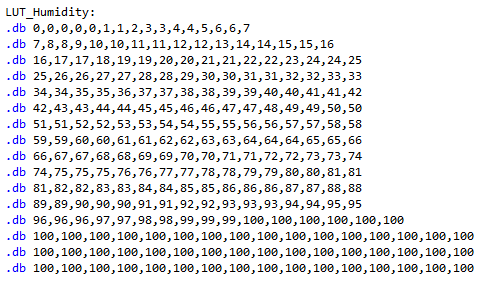
\includegraphics[width=0.7\columnwidth]{LUT.png}
	\caption{Lookup-Tabelle für relative Luftfeuchtigkeit}
\end{figure}
\\
Die erhaltenen Bits kann man jetzt als Index für den entsprechenden Wert der Bitfolge benutzen. Beispielsweise würde jetzt der Wert 1073, welcher mit einer Genauigkeit von 12 Bit gemessen wurde, durch 16 geteilt und als Index verwendet werden (1073/16 = 67). Der 67. Eintrag der Tabelle entspricht dem Wert 35\% (zuvor 35.50\%). Den Verlust der Genauigkeit nehmen wir hier für eine einfache Implementierung in Kauf. Der Zugriff auf den Eintrag erfolgt über den Befehl \texttt{lpm}. Dazu wird zunächst die Adresse der Tabelle um eine Stelle nach links verschoben in den Z Pointer geladen und auf die Adresse der Index addiert, um beim Verwenden von \texttt{lpm} den richtigen Eintrag zu laden.

\subsection{Ausgabe über UART}

\subsection{Interrupts}

\subsection{Zusätzlich}

\section{Schwierigkeiten}
\begin{itemize}
	\item Ground nicht angeschlossen
	\item Stromstecker vergessen
	\item Fehler ohne Debugger zu finden -> Lösungsansatz mit Oszilloskop oder an bestimmten Stellen vom Code LED zum leuchten bringen (um auch zu sehen ob man bestimmte Codeblöcke erreicht - in der richtigen Reihenfolge erreicht)
	\item AtmelStudio STK 500 hinzufügen - allgemein einen funktionierenden Programmer haben - Diamex dann auch mit richtigen Switches auf ON 
\end{itemize}

\end{document}